% Provenance (never printed): see sources/outline_sources.md (Year 2: oceanic islands; growth,
% flank collapse and erosion of volcanic islands; reefs and atolls; subsidence). Hawaiian
% stages, slides, subsidence and drowned reefs after Clague and Sherrod (2014, USGS PP 1801
% ch. 3) and Denlinger and Morgan (2014, ch. 4); the Nuuanu slide after the ODP Leg 200 report;
% the Enewetak holes after Ladd and Schlanger (1960, USGS PP 260-Y); Kure after the NOAA
% monument pages; the depth--age law from the Book 2 and Book 3 rows. Curves and the invented
% Petrel island from figdata/bachelor-2/islands.py; exercise and problem values in the Book 4
% scratch calculator calc/ch17.py.
\chapter{Ilhas oceânicas}\label{ch:b2:oceanic-islands}

Em 1952, em duas ilhas do \omterm{def:b2:oceanic-islands:reefs}{atol} de Enewetak, no Pacífico ocidental (então grafado Eniwetok), dois
furos de sondagem desceram através de rocha coralina até mais de \qty{1.2}{km}. Na ilha Parry, a broca
trouxe fragmentos de basalto fresco a uma profundidade de 4\,158 pés, \qty{1267}{m}, e depois um testemunho de
basalto com olivina. Acima dele havia calcário de idade eocena, cheio de corais recifais de um tipo que não
cresce a mais de cerca de \qty{46}{m} de profundidade. Um recife de coral tinha crescido um dia nos ombros de um vulcão perto do
nível do mar, e o vulcão tinha afundado mais de um quilômetro enquanto o recife continuava crescendo sobre
ele. Este capítulo acompanha uma \omterm{def:b2:oceanic-islands:stages}{ilha oceânica} ao longo de toda a sua vida: como ela cresce, como seus flancos
caem no mar, por que ela afunda, e como um anel de coral pode sobreviver a ela.
% ledger: ls60:enewetak, ics4:eocene

\begin{recall}
\textbf{Do volume do primeiro ano}: ponto quente, pluma mantélica, trilha de ponto quente e sua progressão de idades,
a cadeia Havaí--Imperador e o soerguimento havaiano; a lei profundidade--idade do fundo oceânico; os recifes,
suas formas em franja, em barreira e em \omterm{def:b2:oceanic-islands:reefs}{atol} tal como Darwin as descreveu, e a regra ``acompanhar ou
afogar''; a eustasia e o nível do mar do último máximo glacial, cerca de \qty{120}{m} mais baixo que
hoje. \textbf{Dos volumes escolares}: o vulcão-escudo; a plataforma de abrasão.
\textbf{Do \cref{ch:b2:magmatic-series}}: as \omterm{def:b2:magmatic-series:series}{séries toleítica} e alcalina.
\end{recall}

\section{O crescimento de uma ilha vulcânica}\label{sec:b2:oceanic-islands:growth}

As ilhas havaianas são a extremidade mais jovem da cadeia que o volume do primeiro ano acompanhou através do
Pacífico norte. As ilhas principais contêm 19 vulcões-escudo conhecidos: 15 se elevam acima do mar,
3 estão submersos, e um, recém-nascido, ainda está debaixo d'água. À medida que a placa do Pacífico os leva
para noroeste, cada um nasce acima do ponto quente, cresce, morre ao se afastar, e afunda. A vida é
regular o bastante para ser dividida em fases.
% ledger: cs14:volcanoes

\begin{definition}[Ilha oceânica; fases de crescimento]\label{def:b2:oceanic-islands:stages}
Uma \emph{ilha oceânica}\index{ilha oceânica} é uma ilha vulcânica que se eleva do fundo
oceânico, construída sobre litosfera oceânica. Uma ilha de uma cadeia de ponto quente passa por quatro fases
eruptivas: uma fase \emph{pré-escudo}, de pequenas erupções de lava alcalina no fundo do mar; a
\emph{fase de escudo}\index{fase de escudo}, na qual a lava toleítica constrói a maior parte do vulcão
enquanto ele está sobre o ponto quente; uma fase \emph{pós-escudo}, de erupções menos numerosas e mais alcalinas,
que recobrem o escudo; e, depois de uma pausa, uma fase \emph{rejuvenescida}, de erupções alcalinas raras e
pequenas. A erosão e o afundamento então assumem.
\end{definition}
% ledger: usgs14:hawaii-stages, cs14:rejuvenated

As fases seguem o aporte de calor. Loihi, o vulcão mais novo, fica \qty{54}{km} ao sul do
cume do Kilauea; seu topo ainda está \qty{975}{m} abaixo do mar, mas já \qty{2.5}{km} acima do
fundo do mar em volta, e suas lavas mais antigas são alcalinas. Na \omterm{def:b2:oceanic-islands:stages}{fase de escudo}, o vulcão está sobre
o ponto quente e é alimentado à taxa mais alta. Cada vulcão havaiano emite, segundo as estimativas, de 80 a
\qty{95}{\percent} de seu volume final nessa fase, sobretudo nos seus primeiros 1 a \qty{2}{Myr}.
No fim da fase, a taxa de erupção cai por um fator de dez. Os reservatórios magmáticos rasos, de 1
a \qty{7}{km} de profundidade, já não podem ser mantidos vivos, embora outros menores, a 20 a \qty{30}{km},
permaneçam. A lava volta a ser alcalina, porque um grau de fusão menor a produz, como
mostrou o \cref{ch:b2:magmatic-series}. A fase rejuvenescida vem depois de uma pausa de menos de 0.5
a \qty{2.0}{Myr}. Ela pode ser um ou dois episódios, ou muito longa: em Niihau, durou de 2.2 a
\qty{0.4}{Ma}, e em Kauai continua desde \qty{3.5}{Ma}.
% ledger: cs14:loihi, usgs14:hawaii-stages, cs14:rejuvenated

Os volumes são enormes. O volume do Mauna Loa é estimado em cerca de \qty{74000}{km^3}. Quando o limite com o Kilauea é traçado de novo de modo que o Kilauea fique com apenas cerca de
\qty{10000}{km^3}, a parte do Mauna Loa sobe para \qty{95600}{km^3}. O jovem Loihi contém
\qty{1700}{km^3}. A cadeia inteira, desde \qty{81}{Ma}, soma cerca de
\qty{2e6}{km^3}; uma taxa de erupção integrada sobre essa história, \qty{0.07}{km^3} por ano, daria quase três vezes mais. A carga é pesada o bastante para curvar a
placa: a crosta oceânica sob as ilhas é empurrada para baixo em até \qty{5}{km}, ao longo de uma
depressão chamada Fosso Havaiano (Hawaiian Moat), e uma intumescência baixa, o Arco Havaiano, se eleva a algumas centenas de
quilômetros. Como uma placa se curva sob uma carga é tratado no volume do terceiro~ano. Aqui o fosso
importa porque é para onde vai boa parte dos detritos das ilhas.
% ledger: cs14:volumes, cs14:loihi, cs14:moat

\begin{omfigure}
\centering
\begin{tikzpicture}[x=0.95cm, y=0.95cm, font=\footnotesize]
% schematic, not to scale (vertical exaggeration about 10). Sea level y = 0; sea floor
% y = -1.6 - 0.0625 (16 - x), deepening with the age of the plate to the left.
\fill[omSea!45] (0,0) -- (16,0) -- (16,-1.6) -- (0,-2.6) -- cycle;
\fill[black!18] (0,-2.6) -- (16,-1.6) -- (16,-3.1) -- (0,-3.1) -- cycle;
\draw[black!60] (0,-2.6) -- (16,-1.6);
\draw[omSea!60!black] (0,0) -- (16,0);
\node[anchor=south, font=\scriptsize] at (8.7,0) {nível do mar};
% (a) shield stage over the hotspot
\fill[lith basalt, draw=black!70] (12.6,-1.8125) -- (13.9,0.75) -- (14.3,0.9) -- (14.7,0.75) -- (16,-1.6) -- cycle;
% (b) eroded island with a fringing reef (valleys notched in the summit)
\fill[lith basalt, draw=black!70] (9.2,-2.025) -- (10.1,0.15) -- (10.3,0.35) -- (10.45,0.2) -- (10.6,0.45) -- (10.8,0.25) -- (11.0,0.3) -- (11.2,0.1) -- (12.0,-1.85) -- cycle;
\fill[lith reef limestone, draw=black!70] (10.038,0) -- (9.976,-0.15) -- (9.80,0) -- cycle;
\fill[lith reef limestone, draw=black!70] (11.241,0) -- (11.303,-0.15) -- (11.46,0) -- cycle;
% (c) barrier reef around a smaller island, a lagoon between
\fill[lith basalt, draw=black!70] (5.8,-2.2375) -- (7.0,0.2) -- (8.2,-2.0875) -- cycle;
\fill[lith reef limestone, draw=black!70] (6.384,-1.05) -- (6.42,0) -- (6.60,0) -- (6.62,-0.45) -- (6.680,-0.45) -- cycle;
\fill[lith reef limestone, draw=black!70] (7.656,-1.05) -- (7.62,0) -- (7.44,0) -- (7.42,-0.45) -- (7.341,-0.45) -- cycle;
% (d) atoll: volcano bevelled and drowned, reef cap with a lagoon
\fill[lith basalt, draw=black!70] (2.7,-2.43125) -- (3.6,-0.55) -- (4.0,-0.55) -- (4.9,-2.29375) -- cycle;
\fill[lith reef limestone, draw=black!70] (3.4325,-0.9) -- (3.47,0) -- (4.14,0) -- (4.1806,-0.9) -- (4.0,-0.55) -- (3.6,-0.55) -- cycle;
\fill[omSea!45] (3.62,-0.15) rectangle (3.99,0);
% (e) guyot: flat top with a drowned reef cap, beyond the Darwin point
\fill[lith basalt, draw=black!70] (0.2,-2.5875) -- (0.9,-0.95) -- (1.7,-0.95) -- (2.4,-2.475) -- cycle;
\fill[lith reef limestone, draw=black!70] (0.9,-0.95) -- (0.96,-0.75) -- (1.64,-0.75) -- (1.7,-0.95) -- cycle;
% Darwin point
\draw[black!70, dashed] (2.55,0.55) -- (2.55,-2.5);
\node[anchor=south, font=\scriptsize] at (2.55,0.55) {ponto de Darwin};
% hotspot and plate motion
\draw[omThm, line width=1.4pt, -{Stealth[length=2.5mm]}] (14.3,-3.9) -- (14.3,-3.15);
\node[anchor=west, font=\scriptsize, text=omThm] at (14.4,-3.7) {ponto quente};
\draw[black, line width=0.8pt, -{Stealth[length=2.5mm]}] (9.5,-2.85) -- (6.5,-2.85);
\node[anchor=west, font=\scriptsize] at (9.6,-2.85) {movimento da placa};
\node[anchor=west, font=\scriptsize] at (0.1,-2.9) {litosfera oceânica};
% stage labels
\node[align=center, font=\scriptsize] at (14.3,1.45) {(a) fase de escudo};
\node[align=center, font=\scriptsize] at (10.6,1.3) {(b) ilha erodida,\\ recife em franja};
\node[align=center, font=\scriptsize] at (7.0,1.45) {(c) recife em barreira};
\node[align=center, font=\scriptsize] at (3.8,1.45) {(d) atol};
\node[align=center, font=\scriptsize] at (1.3,1.45) {(e) guyot};
\draw[black!60, -{Stealth[length=2mm]}] (13.6,-3.7) -- (0,-3.7);
\node[anchor=south, font=\scriptsize, fill=white, inner sep=1pt] at (7,-3.7) {vulcões mais velhos, placa mais velha e mais profunda};
\end{tikzpicture}
\par\smallskip{\small A vida de uma \omterm{def:b2:oceanic-islands:stages}{ilha oceânica}, lida ao longo de uma cadeia de ponto quente (esquemático, fora de
escala, escala vertical muito exagerada). A placa leva cada vulcão para longe do ponto quente
(à direita) e o vulcão afunda com ela, enquanto a erosão o desgasta. (a)~Um vulcão-escudo cresce sobre
o ponto quente. (b)~Extinto e erodido, ele é orlado por recifes. (c)~Mais afundado, é cercado
por um \omterm{def:b2:oceanic-islands:reefs}{recife em barreira} com uma laguna atrás. (d)~Seu cume desapareceu sob o mar, e uma capa recifal com
uma laguna central, um \omterm{def:b2:oceanic-islands:reefs}{atol}, cresce sobre ele. (e)~Levado para águas frias demais para que o recife
acompanhe, o \omterm{def:b2:oceanic-islands:reefs}{atol} se afoga e afunda como um \omterm{def:b2:oceanic-islands:seamount}{guyot} de topo plano.}
\end{omfigure}
% ledger: cs14:volcanoes, cs14:erase, cs14:darwin-point, pmnm:geology

\section{O colapso de flanco}\label{sec:b2:oceanic-islands:collapse}

Um vulcão de vários quilômetros de altura, construído de derrames de lava soltos e de entulho, apoiado em encostas que
descem para o fosso, não é estável. Em 1975, o terremoto de Kalapana, de magnitude 7.7, deslocou
o flanco sul do Kilauea até \qty{10}{m} em direção ao mar de uma só vez e gerou um tsunami. Em
1868, outro movimento de flanco veio com um terremoto de magnitude 7.9 e um tsunami que matou 46
pessoas. Perfis sísmicos sob esses flancos mostram um refletor profundo. Ele é interpretado como um
\omterm{def:b2:alpine-orogen:decollement}{descolamento} ao longo do topo da antiga crosta oceânica, sobre o qual todo o flanco desliza. Em geral, o
flanco desliza lentamente (\textit{creep}); às vezes, ele se rompe.
% ledger: dm14:flank

\begin{definition}[Colapso de flanco; avalanche de detritos; slump]\label{def:b2:oceanic-islands:collapse}
Um \emph{colapso de flanco}\index{colapso de flanco} é a ruptura de uma grande parte do flanco de um
vulcão, que desliza sob seu próprio peso. Quando a massa em movimento se fragmenta e corre
depressa, como um fluxo de blocos e entulho que pode viajar muito além do pé do vulcão, é uma
\emph{avalanche de detritos}\index{avalanche de detritos}. Quando ela se move devagar, como grandes blocos que giram
sobre falhas enraizadas num \omterm{def:b2:alpine-orogen:decollement}{descolamento} profundo e ficam perto do vulcão, é um \emph{slump}.
\end{definition}

A evidência está sob o mar. No fim dos anos 1980, o mapeamento por sonar de varredura lateral das águas em torno
das ilhas havaianas mostrou detritos espalhados pelo fundo do mar profundo, a várias centenas de quilômetros
das ilhas, e slumps feitos de grandes blocos segmentados. Dezessete grandes deslizamentos foram identificados
em torno das ilhas principais, formados nos últimos \qty{5}{Myr}. Setenta são conhecidos hoje ao longo da
Dorsal Havaiana entre a ilha do Havaí e Midway, formados ao longo de \qty{30}{Myr}. Isso dá pelo
menos um deslizamento a cada \qty{300}{kyr} em torno das ilhas principais. Essas contagens são mínimas, pois um
vulcão mais jovem pode soterrar a cicatriz e os detritos de um mais antigo: a \omterm{def:b2:eruptive-styles:caldera}{caldeira} do cume e uma zona de rifte
de Niihau estão faltando, e nenhum depósito foi encontrado para elas. Os deslizamentos gigantes parecem mais prováveis enquanto o
vulcão cresce mais depressa, do fim da fase pré-escudo ao início da pós-escudo, mas continuam
muito tempo depois.
% ledger: cs14:slides, dm14:flank

O maior é o deslizamento de Nuuanu, que arrancou o flanco nordeste do vulcão
Koolau, em Oahu. É uma \omterm{def:b2:oceanic-islands:collapse}{avalanche de detritos} espalhada por \qty{23000}{km^2}, estendendo-se por mais de
\qty{200}{km} a partir da ilha. Seus blocos incluem o \omterm{def:b2:oceanic-islands:seamount}{monte submarino} Tuscaloosa, com cerca de \qty{30}{km} de comprimento,
\qty{17}{km} de largura e pelo menos \qty{2}{km} de altura. A avalanche atravessou o fosso profundo e subiu
mais de \qty{100}{km} pela encosta do Arco Havaiano. Sua idade é estimada em 2.1 a
\qty{1.8}{Ma}, perto do fim da vida do Koolau ou depois dela, cujas lavas superficiais têm de 1.8 a
\qty{2.6}{Ma}. De quantos colapsos ela foi feita, e qual é sua espessura longe da ilha,
são questões ainda em aberto.
% ledger: odp200:nuuanu

\begin{omfigure}
\centering
\begin{tikzpicture}[x=0.95cm, y=0.95cm, font=\footnotesize]
% schematic section from the summit of an island (left) across the moat to the arch (right);
% not to scale. Sea level y = 0; top of the old oceanic crust, bent down under the island.
\fill[omSea!45] (0,0) -- (15,0) -- (15,-2.2) -- (13.5,-2.12) -- (11,-2.05) -- (8.5,-2.35) -- (6.5,-2.75) -- (5.6,-2.82) -- (4.0,-1.4) -- (2.5,0) -- cycle;
\fill[black!18] (0,-3.05) -- (5.6,-2.82) -- (6.5,-2.75) -- (8.5,-2.35) -- (11,-2.05) -- (13.5,-2.12) -- (15,-2.2) -- (15,-3.6) -- (0,-3.6) -- cycle;
\draw[black!70] (0,-3.05) -- (5.6,-2.82) -- (6.5,-2.75) -- (8.5,-2.35) -- (11,-2.05) -- (13.5,-2.12) -- (15,-2.2);
\draw[omSea!60!black] (0,0) -- (15,0);
\node[anchor=south east, font=\scriptsize] at (15,0) {nível do mar};
% the volcano: present flank (after collapse) and the lost flank (dashed)
\fill[lith basalt, draw=black!70] (0,1.15) -- (0.8,1.05) -- (1.25,0.95) -- (1.45,0.45) -- (1.75,0.1) -- (2.6,-0.75) -- (3.6,-1.6) -- (4.6,-2.4) -- (5.6,-2.82) -- (0,-3.05) -- cycle;
\draw[black!70, dashed] (1.25,0.95) -- (2.5,0) -- (4.0,-1.4) -- (5.6,-2.82);
\node[font=\scriptsize, align=center, fill=white, inner sep=1pt] at (0.8,-1.6) {vulcão};
\node[font=\scriptsize, anchor=south west, align=left] at (2.0,0.25) {cicatriz do\\ flanco perdido};
% slump: blocks rotated on listric faults rooted in the decollement
\draw[black, line width=0.7pt] (1.45,0.45) .. controls (1.7,-1.4) and (2.4,-2.6) .. (3.6,-2.95);
\draw[black, line width=0.7pt] (2.6,-0.75) .. controls (2.8,-1.8) and (3.3,-2.6) .. (4.4,-2.9);
\draw[omThm, line width=1.1pt] (0.6,-3.03) -- (5.6,-2.82);
\node[anchor=north, font=\scriptsize, text=omThm] at (2.9,-3.05) {descolamento};
% debris avalanche: hummocky sheet across the moat and up the arch, with blocks
\fill[lith conglomerate, draw=black!70] (4.6,-2.4) -- (5.6,-2.62) -- (6.5,-2.6) -- (8.5,-2.22) -- (11,-1.95) -- (12.6,-2.03) -- (11,-2.05) -- (8.5,-2.35) -- (6.5,-2.75) -- (5.6,-2.82) -- cycle;
\fill[lith basalt, draw=black!70] (7.0,-2.62) -- (7.25,-2.25) -- (7.95,-2.22) -- (8.1,-2.43) -- cycle;
\fill[lith basalt, draw=black!70] (9.3,-2.2) -- (9.45,-2.02) -- (9.75,-2.0) -- (9.85,-2.17) -- cycle;
\fill[lith basalt, draw=black!70] (10.6,-2.05) -- (10.7,-1.93) -- (10.9,-1.92) -- (10.95,-2.03) -- cycle;
\draw[black!70] (7.6,-2.2) -- (7.4,-1.3) node[anchor=south, font=\scriptsize, align=center] {bloco de vários\\ km};
\node[anchor=south, font=\scriptsize, align=center] at (10.3,-1.3) {avalanche de detritos};
\draw[black!70] (10.3,-1.3) -- (10.0,-1.98);
\node[font=\scriptsize] at (6.6,-3.2) {fosso};
\node[font=\scriptsize] at (11.6,-2.6) {arco};
\node[anchor=west, font=\scriptsize] at (12.6,-3.3) {crosta oceânica};
\draw[black!70] (2.55,-1.55) -- (3.35,-0.6) node[anchor=west, font=\scriptsize, inner sep=1pt] {slump};
\draw[black!60, {Stealth[length=2mm]}-{Stealth[length=2mm]}] (5.6,-3.95) -- (12.6,-3.95);
\node[anchor=north, font=\scriptsize] at (9.1,-3.95) {até cerca de \qty{200}{km}};
\end{tikzpicture}
\par\smallskip{\small \omterm{def:b2:oceanic-islands:collapse}{Colapso de flanco} de uma \omterm{def:b2:oceanic-islands:stages}{ilha oceânica} (esquemático, fora de escala). Perto do
vulcão, um slump se move devagar como blocos que giram sobre falhas enraizadas num \omterm{def:b2:alpine-orogen:decollement}{descolamento} no topo
da antiga crosta oceânica. Uma \omterm{def:b2:oceanic-islands:collapse}{avalanche de detritos} se desprende do flanco, deixando uma cicatriz, e corre como
um lençol de entulho que carrega blocos de vários quilômetros. A avalanche de Nuuanu atravessou o fosso
e subiu no arco, a mais de \qty{200}{km} de Oahu.}
\end{omfigure}
% ledger: dm14:flank, odp200:nuuanu, cs14:moat

Um deslizamento que cai no mar empurra a água para o lado. Em Lanai e Molokai, brechas caóticas
de coral e lava se elevam a até \qty{155}{m} acima do nível do mar e foram interpretadas como os depósitos de
ondas gigantes geradas por colapsos. A interpretação é contestada. Alguns autores explicam os depósitos por um
soerguimento das ilhas, embora recifes afogados ao sul de Lanai não mostrem nenhum sinal desse soerguimento.
Cerca de um terço dos deslizamentos havaianos gigantes foram \omterm{def:b2:oceanic-islands:collapse}{avalanches de detritos} capazes de gerar ondas enormes. Como
se avalia um perigo assim, raro mas muito grande, é uma questão para o \cref{ch:b2:geological-hazards}.
% ledger: cs14:megatsunami

\section{Por que as ilhas oceânicas afundam}\label{sec:b2:oceanic-islands:subsidence}

Dois processos fazem uma \omterm{def:b2:oceanic-islands:stages}{ilha oceânica} afundar, e eles se sobrepõem. O primeiro é a carga: à medida que o vulcão
cresce, seu peso empurra a placa para baixo. Essa fase rápida dura talvez um milhão de anos e
afoga linhas de costa e recifes em mais de um quilômetro. Ao largo da costa noroeste da ilha do
Havaí, recifes afogados datados dão uma taxa de afundamento de \qty{2.6}{m} por mil anos. Um pequeno
vulcão pode se afogar inteiramente nessa fase: Mahukona, ao lado da ilha do Havaí, foi brevemente uma
ilha e hoje tem seu cume a cerca de \qty{1100}{m} debaixo d'água. O segundo processo é o
resfriamento da placa, que continua por cem milhões de anos, e que esta seção põe em
números.
% ledger: cs14:subsidence, cs14:mahukona

O volume do primeiro ano mediu como o fundo oceânico se aprofunda com sua idade $t$ (em \unit{Myr}). Na
forma usada neste capítulo:
\[
d(t) = \qty{2500}{m} + C\sqrt{t}, \qquad C = \qty{350}{m.Myr^{-1/2}}, \qquad 0 \le t \le 70,
\]
e, para placas com mais de cerca de \qty{20}{Myr},
\[
d(t) = \qty{6400}{m} - \qty{3200}{m}\; e^{-t/62.8}.
\]
As duas formas concordam a cerca de \qty{20}{m} entre 20 e \qty{50}{Myr}, e se cruzam em
\qty{26}{Myr}.
% ledger: ps77:depth-age (Book 2), parsons:plate-model (Book 3)
% values (islands.py): t_switch 26.27, d_switch 4293.8; root - exp: 20 Myr -7.6, 50 Myr +18.3

\begin{proposition}[Afundamento térmico de uma ilha]\label{prop:b2:oceanic-islands:sinking}
Uma ilha construída sobre uma placa de idade $t_1$, levada com a placa, carregando-a com um peso que
já não muda e deixando inalterado o resfriamento da placa sob ela, afunda
\[
S = d(t_2) - d(t_1)
\]
até o momento em que a placa atinge a idade $t_2$, à taxa $\dot S = d'(t)$. Com a lei da raiz,
\[
S = C\left(\sqrt{t_2} - \sqrt{t_1}\right), \qquad \dot S = \frac{C}{2\sqrt t},
\]
e, com a lei exponencial, $\dot S = (\qty{3200}{m}/\qty{62.8}{Myr})\,e^{-t/62.8}$. Num
intervalo dado, uma placa jovem leva suas ilhas mais para baixo do que uma placa velha.
\end{proposition}

\begin{proof}
Comparem-se duas colunas da placa, da mesma idade, uma sob a ilha e outra sob o oceano aberto,
longe. As duas se resfriam da mesma maneira, pois a ilha deixa inalterado o resfriamento da placa. Logo as duas se contraem da mesma quantidade, e o topo de cada uma desce da mesma
quantidade. O próprio peso da ilha já está equilibrado e não muda mais, de modo que não acrescenta nada
mais. A coluna do oceano aberto desce $d(t_2) - d(t_1)$; a ilha também. Derivar
dá a taxa. Quanto à última afirmação: num intervalo fixo $\Delta$, $C(\sqrt{t_1 + \Delta} -
\sqrt{t_1})$ diminui quando $t_1$ cresce, pois sua derivada, $\frac C2\bigl(1/\sqrt{t_1 + \Delta}
- 1/\sqrt{t_1}\bigr)$, é negativa.
\end{proof}

A proposição deixa de fora duas coisas de propósito. O soerguimento do ponto quente levanta a placa quando ela
passa e a deixa descer de novo quando ela se afasta, o que se soma ao afundamento das ilhas mais jovens
(o volume do primeiro ano mediu esse soerguimento). E uma carga muda enquanto o vulcão cresce, o que é a
fase rápida acima. Uma vez terminadas as duas, a ilha acompanha o fundo.

As taxas são pequenas. Numa placa de \qty{4}{Myr}, a lei da raiz dá \qty{87.5}{m} por milhão
de anos, menos de um décimo de milímetro por ano. Numa placa de \qty{100}{Myr}, a lei exponencial
dá \qty{10.4}{m} por milhão de anos, ou \qty{0.01}{m} por mil anos. Essa é a taxa
medida ao longo de boa parte da Dorsal Havaiana e dos \omterm{def:b2:oceanic-islands:seamount}{montes submarinos} do Imperador. A fase de carga, a
\qty{2.6}{m} por mil anos, é umas 250 vezes mais rápida.
% ledger: cs14:subsidence; values (islands.py): rate_100 10.37, age_rate10 102.3

\begin{omfigure}
\centering
% figdata/bachelor-2/islands.py part sink
\begin{tikzpicture}
\begin{axis}[width=0.8\linewidth, height=6.2cm, y dir=reverse, xmin=0, xmax=100, ymin=0,
  ymax=3000, xlabel={tempo desde a construção da ilha (\unit{Myr})},
  ylabel={afundamento térmico (\unit{m})}, tick label style={font=\scriptsize},
  label style={font=\small}, xtick pos=bottom, ytick pos=left]
\addplot[omThm, line width=1pt] table[x=dt_Myr, y=t2] {figdata/out/bachelor-2-islands-sink.dat};
\addplot[orange!80!black, line width=1pt] table[x=dt_Myr, y=t10] {figdata/out/bachelor-2-islands-sink.dat};
\addplot[blue!70!black, line width=1pt] table[x=dt_Myr, y=t30] {figdata/out/bachelor-2-islands-sink.dat};
\addplot[black!45, line width=1pt] table[x=dt_Myr, y=t60] {figdata/out/bachelor-2-islands-sink.dat};
\node[font=\scriptsize, anchor=south east, inner sep=1pt] at (axis cs:99,2470) {placa de \qty{2}{Myr}};
\node[font=\scriptsize, anchor=south east, inner sep=1pt] at (axis cs:99,2140) {\qty{10}{Myr}};
\node[font=\scriptsize, anchor=south east, inner sep=1pt] at (axis cs:99,1380) {\qty{30}{Myr}};
\node[font=\scriptsize, anchor=south east, inner sep=1pt] at (axis cs:99,710) {\qty{60}{Myr}};
\draw[black!50, dashed] (axis cs:0,1267) -- (axis cs:58,1267);
\node[font=\scriptsize, anchor=north west, inner sep=1pt] at (axis cs:1,1300) {Enewetak, \qty{1267}{m}};
\end{axis}
\end{tikzpicture}
\par\smallskip{\small Afundamento térmico de uma ilha levada por sua placa, a partir da lei profundidade--idade,
para ilhas construídas sobre placas de 2, 10, 30 e \qty{60}{Myr} (a lei da raiz até uma idade da placa de
\qty{26}{Myr}, a lei exponencial além, onde as duas se encontram). Quanto mais jovem a placa, mais depressa
e mais longe a ilha afunda. A linha tracejada marca a profundidade do basalto sob Enewetak, a
espessura de rocha recifal para a qual o afundamento tem de abrir espaço.}
\end{omfigure}
% ledger: ps77:depth-age (Book 2), parsons:plate-model (Book 3), ls60:enewetak

\section{Recifes, atóis e guyots}\label{sec:b2:oceanic-islands:reefs}

O volume do primeiro ano descreveu as três formas de recife tal como Darwin as explicou, de um recife que orla
uma ilha a um anel de coral em torno de uma laguna, e terminou numa pergunta: por que as ilhas afundam,
e até onde? A seção anterior a respondeu. As formas podem agora ser definidas pelo estado da
ilha por baixo.

\begin{definition}[Recife em franja; recife em barreira; atol]\label{def:b2:oceanic-islands:reefs}
Um \emph{recife em franja}\index{recife em franja} é um recife preso à costa de uma ilha, sem
laguna, ou apenas com um canal estreito e raso, entre eles. Um \emph{recife em barreira}\index{recife em barreira}
é um recife separado da costa por uma laguna, nos flancos de uma ilha que afundou enquanto o
recife crescia para cima. Um \emph{atol}\index{atol} é um anel de recife, com ilhas baixas de detritos recifais,
em torno de uma laguna sem rocha vulcânica acima do nível do mar: seu vulcão está inteiramente sob o recife.
\end{definition}

\begin{definition}[Monte submarino; guyot]\label{def:b2:oceanic-islands:seamount}
Um \emph{monte submarino}\index{monte submarino} é um vulcão no fundo oceânico cujo cume fica abaixo do nível
do mar, seja porque nunca atingiu a superfície, seja porque afundou. Um
\emph{guyot}\index{guyot} é um monte submarino de topo plano, cortado pelas ondas ou coberto por um recife quando
estava ao nível do mar, e depois afogado.
\end{definition}

Se um recife mantém seu topo ao nível do mar enquanto o vulcão afunda sob ele, a rocha recifal se empilha tão
depressa quanto a ilha desce. A espessura da capa registra então o afundamento.

\begin{proposition}[Espessura de uma capa recifal]\label{prop:b2:oceanic-islands:cap}
Suponha-se que a última rocha vulcânica de uma ilha desça abaixo do nível do mar quando sua placa tem a idade $t_1$, e que um
recife mantenha seu topo ao nível do mar desde então, até que a placa tenha a idade $t_2$. Se o nível do mar subiu
de $\Delta\eta$ entre os dois momentos (em relação ao centro da Terra), então a capa recifal
sobre o vulcão tem
\[
H = d(t_2) - d(t_1) + \Delta\eta = C\left(\sqrt{t_2} - \sqrt{t_1}\right) + \Delta\eta
\]
de espessura, a segunda forma com a lei da raiz. Ela não depende da taxa à qual o recife pode
crescer, desde que essa taxa nunca seja menor que a subida relativa do nível do mar.
\end{proposition}

\begin{proof}
Em $t_1$, o topo do vulcão está ao nível do mar; em $t_2$, ele está $S = d(t_2) - d(t_1)$ mais baixo pela
\cref{prop:b2:oceanic-islands:sinking}, enquanto a superfície do mar subiu de $\Delta\eta$. O topo
do recife está na superfície do mar nos dois momentos, e sua base é o topo do vulcão. Logo a
espessura é a distância entre eles, $S + \Delta\eta$. Um recife que acompanha para na
superfície, de modo que um recife mais rápido não constrói uma capa mais espessa; um recife que não consegue acompanhar fica para trás
e se afoga, que é a regra lembrada do volume do primeiro ano.
\end{proof}

Enewetak confirma isso. Pela lei da raiz, uma capa de \qty{1267}{m} exige $\sqrt{t_2} - \sqrt{t_1} =
1267/350 = 3.62$: por exemplo, um vulcão aplainado ao nível do mar numa placa de \qty{10}{Myr} e
levado até que a placa tenha \qty{46}{Myr}. São \qty{36}{Myr}, a ordem do tempo que
separa a base eocena do calcário de hoje. Os furos também mostraram o que a
proposição deixa de fora. Zonas lixiviadas, onde a aragonita dos corais foi dissolvida ou
recristalizada, registram épocas em que o topo do \omterm{def:b2:oceanic-islands:reefs}{atol} esteve acima do mar e a chuva caiu sobre ele.
O nível do mar desce e sobe com as glaciações, e a capa foi exposta e afogada de novo muitas
vezes em sua descida.
% ledger: ls60:enewetak, ics4:eocene; calc/ch17.py: (3.162 + 3.620)^2 = 46.0

\begin{history}[Perfurar atóis, 1896--1952]
A teoria de Darwin fazia uma previsão que só podia ser verificada com uma sonda: sob um \omterm{def:b2:oceanic-islands:reefs}{atol} deveria
haver uma espessa pilha de rocha recifal de águas rasas, repousando sobre rocha vulcânica. O primeiro furo profundo
num \omterm{def:b2:oceanic-islands:reefs}{atol} do Pacífico foi perfurado em Funafuti de 1896 a 1898 e parou a 1\,114 pés,
\qty{340}{m}, sem atingir o vulcão. Um furo em Kita-daito-jima, ao sul do Japão e a leste de Okinawa,
chegou a 1\,416 pés em 1936, e outro em Bikini a 2\,556 pés em 1947, sem que nenhum deles o atingisse. Os furos de Enewetak, em
1951 e 1952, foram os primeiros a atingir o alicerce de um \omterm{def:b2:oceanic-islands:reefs}{atol}. Em Elugelab, o embasamento duro foi
encontrado a 4\,610 pés; na ilha Parry, o basalto a 4\,158 pés, 450 pés mais acima, a \num{22}~milhas
de distância. Os perfuradores tinham encontrado um vulcão basáltico que se eleva duas milhas acima do fundo oceânico, coberto
por calcário recifal desde o Eoceno. Elugelab foi destruída num teste de um artefato termonuclear
pouco depois do fim da perfuração.
\end{history}
% ledger: ls60:holes, ls60:enewetak

\begin{omfigure}
\centering
% figdata/bachelor-2/islands.py part holes
\begin{tikzpicture}
\begin{axis}[width=0.8\linewidth, height=6.0cm, ybar, bar width=16pt, y dir=reverse, ymin=0,
  ymax=1500, enlarge x limits=0.1, symbolic x coords={Funafuti,Kita-daito-jima,Bikini,Eniwetok-K-1B,Eniwetok-F-1,Eniwetok-E-1},
  xtick=data, xticklabels={{Funafuti\\1898},{Kita-daito-jima\\1936},{Bikini\\1947},{Enewetak\\K-1B, 1951},{Enewetak\\F-1, 1952},{Enewetak\\E-1, 1952}},
  xticklabel style={align=center, font=\scriptsize}, ylabel={profundidade (\unit{m})},
  tick label style={font=\scriptsize}, label style={font=\small}, xtick pos=bottom, ytick pos=left]
\addplot[fill=omLithLime, draw=black!70] table[x=name, y=td_m] {figdata/out/bachelor-2-islands-holes.dat};
\addplot[only marks, mark=-, mark size=9pt, line width=2.2pt, black, unbounded coords=discard, xshift=0pt]
  table[x=name, y=basalt_m] {figdata/out/bachelor-2-islands-holes.dat};
\end{axis}
\end{tikzpicture}
\par\smallskip{\small Os furos profundos perfurados em \omterm{def:b2:oceanic-islands:reefs}{atóis} do Pacífico, com o ano em que cada um foi concluído:
sua profundidade total (barras) e, em Enewetak, a profundidade do embasamento basáltico (marcas pretas)
(\qty{1405}{m} sob Elugelab, F-1; \qty{1267}{m} sob a ilha Parry, E-1). Profundidades convertidas
dos pés do relatório de perfuração.}
\end{omfigure}
% ledger: ls60:holes, ls60:enewetak; values (islands.py): td and basalt in m

\begin{inthefield}[Perfurar um atol]
Em Enewetak, os geólogos situaram os furos profundos perto da margem da laguna, onde esperavam
menos cavernas do que perto da borda externa do recife. A maior parte do furo foi perfurada diretamente, com a rocha triturada em
fragmentos que o fluido de perfuração trazia à superfície. Os fragmentos subiam com atraso, por isso a equipe estimou esse
atraso para saber de que profundidade vinha cada amostra. Em profundidades escolhidas, um barrilete retirava um cilindro
sólido de rocha. Terminada a perfuração, os furos foram usados como instrumentos. Num deles, revestido
até \qty{600}{m}, o nível da água ainda subia e descia com a maré do oceano, em fase e
na mesma amplitude: o calcário da capa é poroso e cheio de cavernas de alto a baixo. Em outros,
mediu-se a temperatura à medida que ela voltava ao equilíbrio.
\end{inthefield}
% ledger: ls60:methods, ls60:casing (F-1 cased to 1,973 ft = 601 m)

Um recife não está fadado a se afogar porque sua ilha afunda. Corais e algas coralinas constroem
milímetros por ano: num estudo moderno, recifes dominados por corais ramificados cresceram \qty{4.2}{mm} por
ano. A
placa que se resfria leva no máximo um décimo de milímetro por ano. O afundamento térmico sozinho nunca
ultrapassará um recife saudável. Os recifes se afogam quando outra coisa muda: a placa os leva para águas
frias demais para um crescimento rápido; o nível do mar sobe mais depressa do que eles conseguem acompanhar; ou as duas coisas ao mesmo tempo.
% ledger: perry:chagos (Book 3), cs14:darwin-point

\begin{omfigure}
\centering
% figdata/bachelor-2/islands.py part rates; horizontal lines from the ledger rows
\begin{tikzpicture}
\begin{semilogyaxis}[width=0.8\linewidth, height=6.4cm, xmin=0, xmax=150, ymin=0.005, ymax=100,
  xlabel={idade da placa (\unit{Myr})}, ylabel={taxa (\unit{mm.yr^{-1}})},
  tick label style={font=\scriptsize}, label style={font=\small}, xtick pos=bottom, ytick pos=left]
\addplot[omThm, line width=1.1pt] table[x=t_Myr, y=thermal_mm_yr] {figdata/out/bachelor-2-islands-rates.dat};
\draw[omThm, densely dotted, line width=0.9pt] (axis cs:75,0.01) -- (axis cs:150,0.01);
\node[font=\scriptsize, anchor=south west, inner sep=1pt, text=omThm] at (axis cs:22,0.042) {afundamento térmico da placa};
\node[font=\scriptsize, anchor=south west, inner sep=1pt, text=omThm] at (axis cs:96,0.0108) {medido, Dorsal Havaiana};
\draw[black!70, line width=0.9pt] (axis cs:0,2.6) -- (axis cs:150,2.6);
\node[font=\scriptsize, anchor=north west, inner sep=1pt] at (axis cs:2,2.6) {carga, ao largo da ilha do Havaí};
\draw[green!50!black, line width=0.9pt] (axis cs:0,4.2) -- (axis cs:150,4.2);
\node[font=\scriptsize, anchor=south west, inner sep=1pt, text=green!40!black] at (axis cs:2,4.2) {crescimento de um recife produtivo};
\draw[blue!70!black, line width=0.9pt] (axis cs:0,12) -- (axis cs:150,12);
\node[font=\scriptsize, anchor=south west, inner sep=1pt, text=blue!70!black] at (axis cs:2,12) {subida média do nível do mar na última deglaciação};
\draw[blue!70!black, line width=0.9pt, dashed] (axis cs:0,40) -- (axis cs:150,40);
\node[font=\scriptsize, anchor=south west, inner sep=1pt, text=blue!70!black] at (axis cs:2,40) {Meltwater Pulse 1A, no mínimo};
\end{semilogyaxis}
\end{tikzpicture}
\par\smallskip{\small As taxas que decidem se um recife acompanha, em escala logarítmica. O
afundamento térmico da placa (a partir da lei profundidade--idade) é dezenas a centenas de vezes mais lento que o
crescimento do recife; a linha pontilhada é a taxa medida ao longo de boa parte da Dorsal Havaiana. O afundamento de um vulcão em crescimento
sob sua própria carga, e sobretudo a subida do nível do mar no fim de uma glaciação, se aproximam
do crescimento de um recife ou o ultrapassam.}
\end{omfigure}
% ledger: cs14:subsidence, perry:chagos (Book 3), lambeck14:lgm (Book 2), ipcc:lgm-sea (Book 2)

\begin{definition}[Ponto de Darwin]\label{def:b2:oceanic-islands:darwin-point}
O \emph{ponto de Darwin}\index{ponto de Darwin} de uma cadeia de ponto quente é o lugar, e o tempo depois
do nascimento dos vulcões, em que o crescimento dos recifes para cima, que se desacelera em águas mais frias,
já não compensa o afundamento das ilhas. Os \omterm{def:b2:oceanic-islands:reefs}{atóis} levados além dele se afogam e se tornam
\omterm{def:b2:oceanic-islands:seamount}{guyots}.
\end{definition}

Na cadeia havaiana, os recifes se afogam cerca de \qty{33}{Myr} depois do nascimento de seu vulcão. O \omterm{def:b2:oceanic-islands:reefs}{atol} de Kure,
na extremidade noroeste das ilhas, é o \omterm{def:b2:oceanic-islands:reefs}{atol} de coral mais setentrional do mundo, e
fica no \omterm{def:b2:oceanic-islands:darwin-point}{ponto de Darwin}. Seu recife ainda cresce um pouco mais depressa do que o \omterm{def:b2:oceanic-islands:reefs}{atol} afunda. Todos os
vulcões além de Midway e Kure estão submersos, e a maioria são \omterm{def:b2:oceanic-islands:seamount}{guyots}. No \omterm{def:b2:oceanic-islands:seamount}{monte submarino} Koko, no
sul da cadeia do Imperador, carbonato foi depositado de cerca de 50 a \qty{16}{Ma}. Depois, as últimas
algas coralinas de águas profundas afundaram abaixo de seu limite de crescimento, cerca de \qty{150}{m} sob o mar. A água
mais fria sozinha não afoga os recifes, nem o afundamento sozinho. O afogamento exige o afundamento,
a deriva para o norte em águas mais frias e mudanças rápidas do clima ao mesmo tempo.
% ledger: cs14:darwin-point, pmnm:kure, pmnm:geology

\begin{omfigure}
\centering
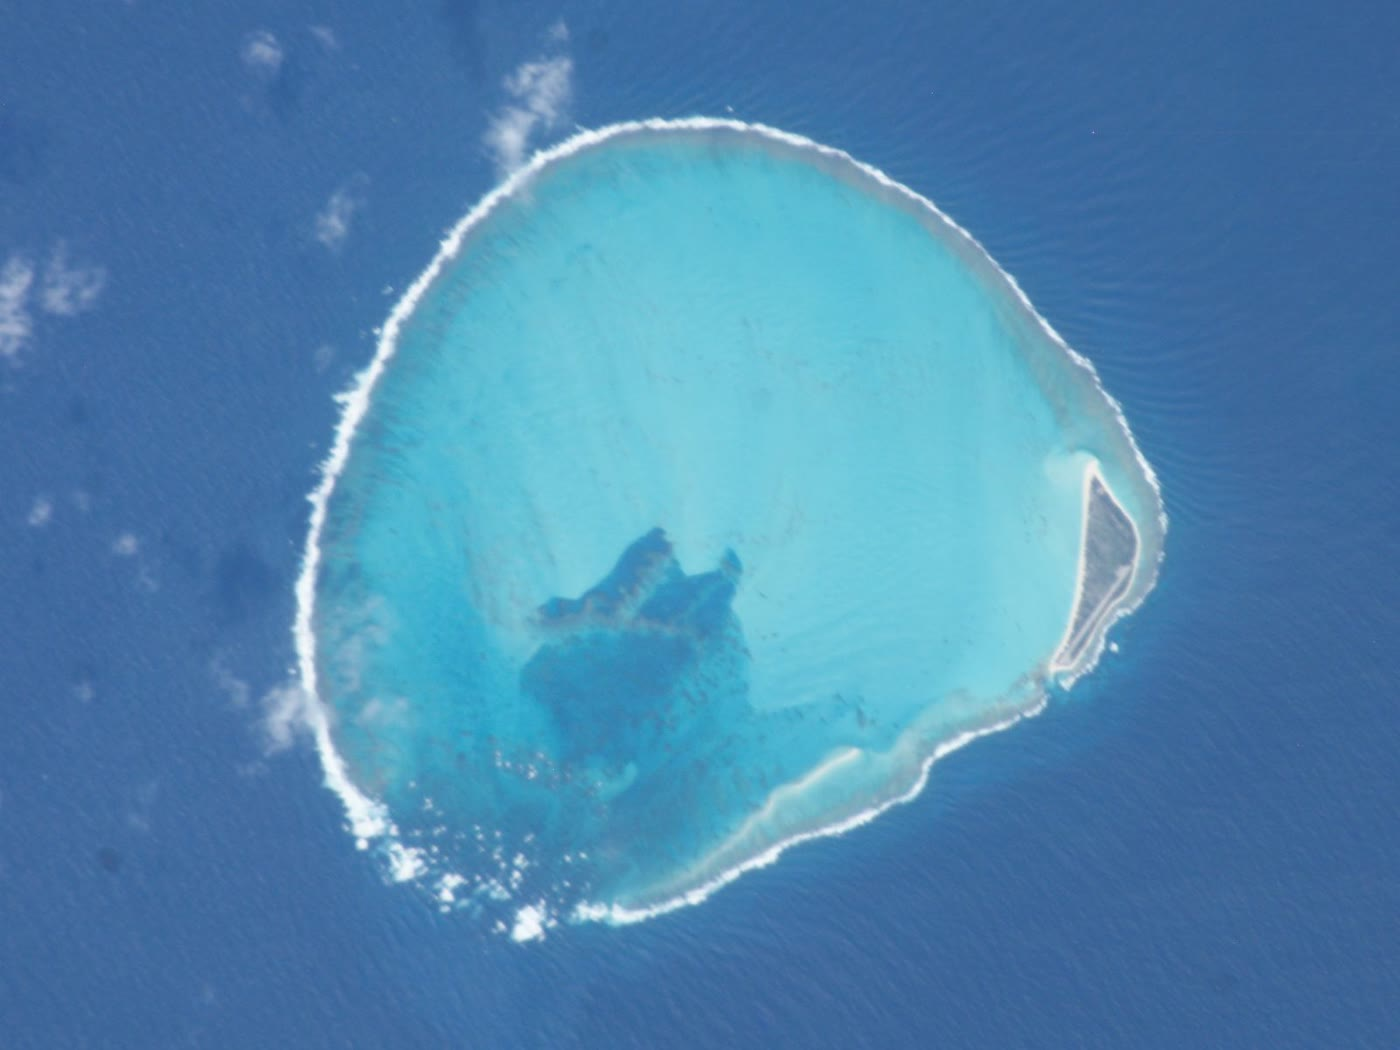
\includegraphics[width=0.52\linewidth]{images/book4/b2-17-kure-atoll.jpg}
\par\smallskip{\small O \omterm{def:b2:oceanic-islands:reefs}{atol} de Kure, o \omterm{def:b2:oceanic-islands:reefs}{atol} de coral mais setentrional, fotografado por um astronauta da
Estação Espacial Internacional em 22 de fevereiro de 2004. O anel de recife, com no máximo cerca de dez quilômetros de diâmetro,
encerra uma laguna; a única ilha permanente, Green Island, fica na borda (à direita). NASA,
domínio público, via Wikimedia Commons.}
\end{omfigure}
% ledger: pmnm:kure (6 miles = 9.7 km)

\section{Erosão, nível do mar e o fim de uma ilha}\label{sec:b2:oceanic-islands:erosion}

Enquanto afunda, uma ilha também é desgastada. Uma ilha alta capta os ventos alísios: nas
encostas a barlavento dos vulcões havaianos, mais de \qty{9}{m} de chuva caem por ano em alguns lugares.
Os rios cavam cânions profundos em menos de um milhão de anos, como no Kohala, na ilha do Havaí.
Algumas grandes falésias antes tidas como obra apenas da erosão, como as falésias marinhas do norte de
Molokai, são hoje interpretadas como as escarpas de cabeceira de deslizamentos gigantes, recuadas desde então. As ondas atacam a costa e
aplainam uma plataforma de abrasão ao nível do mar em volta dela. Erosão e afundamento juntos removem todo vestígio
de rocha vulcânica acima do mar em cerca de \qty{15}{Myr}. Gardner Pinnacles, mais ou menos dessa idade, é
a ilha mais antiga da cadeia onde rocha vulcânica ainda se eleva acima da água. Além dela, para
noroeste, há apenas ilhas de areia, \omterm{def:b2:oceanic-islands:reefs}{atóis} e vulcões afogados.
% ledger: cs14:erosion, cs14:erase

O nível do mar não fica parado enquanto isso acontece. Durante o último máximo glacial, ele estava cerca de
\qty{120}{m} mais baixo que hoje. A costa de uma ilha ficava então mais abaixo em seus flancos, e os recifes
que hoje a orlam eram terra firme. Quando o gelo derreteu, o mar subiu em média \qty{12}{m}
a cada mil anos durante a deglaciação principal, de 16.5 a \qty{8.2}{ka}. Durante o Meltwater
Pulse 1A, ele subiu pelo menos \qty{40}{mm} por ano. Um recife num vulcão que afunda deve acompanhar as duas
subidas. Ao largo da costa noroeste da ilha do Havaí, pelo menos seis recifes afogados formam uma
escadaria no flanco, o mais antigo o mais profundo. Cada um cresceu na costa, ficou para trás durante uma subida
do mar, e foi levado para baixo pela carga da jovem ilha. Uma vez que um vulcão tenha afundado mais
de cerca de \qty{125}{m}, a amplitude do nível do mar glacial, ele não voltará às ondas.
% ledger: usgs:lgm (Book 1), lambeck14:lgm (Book 2), cs14:erase, cs14:subsidence

O arco pode agir no sentido inverso. Oahu está sobre a intumescência levantada pela carga das ilhas mais jovens,
e subiu um pouco: recifes do último interglacial, de 133 a \qty{115}{ka}, afloram em toda a
volta da ilha, e um recife de cerca de \qty{334}{ka} está hoje \qty{21}{m} acima do nível do mar. O
fim de uma \omterm{def:b2:oceanic-islands:stages}{ilha oceânica} está assim escrito em suas rochas e em seus recifes. A lava a constrói, os deslizamentos e
a chuva a desgastam, as ondas a aplainam, a placa a leva para baixo, e um recife mantém seu lugar na
superfície até que a água fria e um mar que sobe o afoguem também.
% ledger: cs14:arch

\section*{Exercícios}\label{sec:b2:oceanic-islands:exercises}

Dados para os exercícios, salvo indicação contrária: lei profundidade--idade $d = \qty{2500}{m} + C\sqrt t$ com
$C = \qty{350}{m.Myr^{-1/2}}$ para $0 \le t \le \qty{70}{Myr}$, e $d = \qty{6400}{m} -
\qty{3200}{m}\,e^{-t/62.8}$ além de \qty{20}{Myr}; $1~\text{pé} = \qty{0.3048}{m}$, $1~\text{braça}
= \qty{1.8288}{m}$, $1~\text{milha} = \qty{1.609}{km}$; crescimento dos recifes até \qty{4.2}{mm.yr^{-1}}.

\begin{exercise}[$\star$]\label{exo:b2:oceanic-islands:1}
Dê a fase de cada vulcão: (a) um \omterm{def:b2:oceanic-islands:seamount}{monte submarino} cujo cume está \qty{975}{m} abaixo do mar, emitindo
lava alcalina; (b) um vulcão sobre o ponto quente, emitindo lava toleítica a uma taxa alta; (c) um
vulcão extinto cujos últimos derrames, mais alcalinos que o grosso da ilha, recobrem o escudo; (d) uma
ilha onde, depois de um silêncio de \qty{2}{Myr}, algumas pequenas bocas alcalinas se abrem; (e) um anel de recife
em torno de uma laguna sem nenhuma rocha vulcânica à vista.
\end{exercise}

\begin{exercise}[$\star$]\label{exo:b2:oceanic-islands:2}
Um vulcão é construído sobre uma placa de \qty{9}{Myr}. (a) Que profundidade tem o fundo do mar em volta dele? (b) Quanto
ele terá afundado quando a placa tiver \qty{25}{Myr}? (c) A que taxa ele afunda então?
\end{exercise}

\begin{exercise}[$\star$]\label{exo:b2:oceanic-islands:3}
Dezessete grandes deslizamentos se formaram nos últimos \qty{5}{Myr} em torno das ilhas havaianas principais, e
setenta ao longo da Dorsal Havaiana em \qty{30}{Myr}. (a) Encontre o intervalo médio entre dois deslizamentos em
cada caso. (b) Por que os dois são apenas limites superiores do intervalo verdadeiro?
\end{exercise}

\begin{exercise}[$\star$]\label{exo:b2:oceanic-islands:4}
Em Enewetak, o basalto foi encontrado a 4\,158 pés num furo e o embasamento duro a 4\,610 pés no
outro; os corais recifais da base do calcário não vivem a mais de 150 pés de profundidade. (a) Converta
as três profundidades em metros. (b) De pelo menos quanto o topo do vulcão sob a ilha Parry
afundou desde que o primeiro recife cresceu sobre ele? (c) A base do calcário é eocena, portanto com pelo menos
\qty{33.9}{Myr}. Qual é a maior taxa média de afundamento possível?
\end{exercise}

\begin{exercise}[$\star\star$]\label{exo:b2:oceanic-islands:5}
(a) Encontre a taxa de afundamento térmico, em \unit{m} por \unit{Myr} e em \unit{mm.yr^{-1}}, de
ilhas sobre placas de 4, 25 e \qty{49}{Myr}. (b) Quantas vezes mais depressa que a mais rápida dessas
um recife produtivo pode crescer? (c) E quantas vezes mais rápida é a fase de carga ao largo da ilha do
Havaí, \qty{2.6}{m} por mil anos?
\end{exercise}

\begin{exercise}[$\star\star$]\label{exo:b2:oceanic-islands:6}
(a) Com a lei exponencial, encontre a taxa de afundamento numa placa de \qty{100}{Myr}, em \unit{m}
por mil anos, e compare-a com os \qty{0.01}{m} por mil anos medidos ao longo da
Dorsal Havaiana. (b) Em que idade da placa a taxa é exatamente \qty{10}{m.Myr^{-1}}? (c) Verifique que as
duas leis dão quase a mesma profundidade para uma placa de \qty{25}{Myr}.
\end{exercise}

\begin{exercise}[$\star\star$]\label{exo:b2:oceanic-islands:7}
Os recifes havaianos se afogam cerca de \qty{33}{Myr} depois do nascimento de seu vulcão, e o vulcanismo se desloca
ao longo da cadeia a \qty{8.6}{cm.yr^{-1}}. (a) A que distância do ponto quente fica uma ilha quando seu
recife se afoga? (b) Midway é um \omterm{def:b2:oceanic-islands:reefs}{atol} de \qty{27.7}{Myr}: é coerente que ele ainda tenha um
recife vivo? (c) Kure fica 55 milhas além de Midway. Estime sua idade, e diga se ele está perto
do \omterm{def:b2:oceanic-islands:darwin-point}{ponto de Darwin}.
\end{exercise}

\begin{exercise}[$\star\star$]\label{exo:b2:oceanic-islands:8}
Na \omterm{def:b2:oceanic-islands:collapse}{avalanche de detritos} de Nuuanu, o \omterm{def:b2:oceanic-islands:seamount}{monte submarino} Tuscaloosa é um bloco de cerca de \qty{30}{km} de comprimento,
\qty{17}{km} de largura e pelo menos \qty{2}{km} de altura. (a) Que volume teria uma caixa com essas dimensões?
E uma pirâmide com a mesma base e a mesma altura? (b) Compare com o volume do
Kilauea, \qty{10000}{km^3}. (c) A avalanche cobre \qty{23000}{km^2}. Se ela tivesse em média
\qty{100}{m} de espessura (uma hipótese: sua espessura longe de Oahu é mal conhecida), qual seria seu
volume?
\end{exercise}

\begin{exercise}[$\star\star$]\label{exo:b2:oceanic-islands:9}
Ao largo da ilha do Havaí, o flanco afunda \qty{2.6}{m} por mil anos sob a carga do
vulcão. (a) Quanto tempo leva para afogar uma linha de costa em \qty{1}{km}? (b) Um recife que cresce a
\qty{4.2}{mm.yr^{-1}} está sobre esse flanco. Ele acompanha quando o nível do mar está estável? (c) Durante a
deglaciação principal, de 16.5 a \qty{8.2}{ka}, o mar subiu em média \qty{12}{mm.yr^{-1}}. A que
profundidade fica o topo do recife no fim, se ele começou na superfície? (d) O mesmo, para um recife sobre
um vulcão antigo que já não afunda.
\end{exercise}

\begin{exercise}[$\star\star\star$]\label{exo:b2:oceanic-islands:10}
(a) Mostre que, num intervalo fixo $\Delta$, a lei da raiz faz uma ilha afundar menos quanto mais velha for sua
placa. (b) Calcule o afundamento em \qty{20}{Myr} para uma ilha nascida na dorsal e para outra nascida
numa placa de \qty{50}{Myr}. (c) A placa sob uma dorsal é muito quente, e a lei da raiz dá uma
taxa infinita em $t = 0$. Isso é um problema para o afundamento num intervalo finito? Explique.
\end{exercise}

\begin{exercise}[$\star\star\star$]\label{exo:b2:oceanic-islands:11}
Um \omterm{def:b2:oceanic-islands:reefs}{atol} afunda a \qty{30}{m.Myr^{-1}}, e o nível do mar oscila cerca de \qty{120}{m} com as
glaciações, em ciclos de cerca de \qty{100}{kyr}. (a) Quanto o \omterm{def:b2:oceanic-islands:reefs}{atol} afunda durante um ciclo? (b) Num
nível baixo glacial, a que altura o topo do \omterm{def:b2:oceanic-islands:reefs}{atol} fica acima do mar? O que acontece então com a
rocha recifal? (c) Quantos ciclos são necessários para que o \omterm{def:b2:oceanic-islands:reefs}{atol} afunde os \qty{120}{m} inteiros?
(d) Explique as zonas lixiviadas encontradas nos furos de Enewetak, e por que a
\cref{prop:b2:oceanic-islands:cap} ainda dá a espessura da capa a longo prazo.
\end{exercise}

\begin{exercise}[$\star\star\star$]\label{exo:b2:oceanic-islands:12}
Um \omterm{def:b2:oceanic-islands:reefs}{atol} se afoga quando sua placa tem \qty{50}{Myr}: seu recife fica para trás e seu topo termina no
limite de crescimento das algas coralinas mais profundas, \qty{150}{m} sob o mar. (a) Com a lei
exponencial, quanto mais ele afunda antes que a placa tenha \qty{120}{Myr}? (b) A que profundidade fica o topo
do \omterm{def:b2:oceanic-islands:seamount}{guyot} então? (c) Um \omterm{def:b2:oceanic-islands:seamount}{guyot} ao lado de Enewetak tem seu topo a 700 braças. Converta, e compare.
(d) Dê duas razões pelas quais um \omterm{def:b2:oceanic-islands:seamount}{guyot} real poderia ser mais profundo ou mais raso que essa estimativa.
\end{exercise}

\begin{problem}[{Problema de fim de semana --- do vulcão ao atol}]\label{pb:b2:oceanic-islands:1}
A ilha Petrel, inventada, nasce sobre um ponto quente numa placa de \qty{10}{Myr}. Seu vulcão é
um cone de raio basal \qty{50}{km}. Quando seu crescimento termina, seu cume está \qty{1000}{m} acima do
nível do mar. Sua última rocha vulcânica desaparece abaixo do nível do mar \qty{12}{Myr} depois. Um recife então
mantém seu topo ao nível do mar até que a placa tenha \qty{70}{Myr}, quando o \omterm{def:b2:oceanic-islands:reefs}{atol} cruza o
\omterm{def:b2:oceanic-islands:darwin-point}{ponto de Darwin}. Use a lei profundidade--idade dos exercícios (a lei da raiz até \qty{70}{Myr}, a
lei exponencial além), um crescimento recifal de \qty{4.2}{mm.yr^{-1}} e os dados do capítulo.
O nível do mar é tomado como constante, exceto nas questões 8 a 10. Arredonde as profundidades ao metro.

\noindent\textbf{Parte I --- Crescimento.}
\begin{enumerate}
  \item Que profundidade tem o fundo do mar onde Petrel nasce?
  \item Qual é a altura do vulcão acima desse fundo quando seu crescimento termina, desprezando o
        afundamento do fundo sob a carga?
  \item Encontre o volume do cone.
  \item Se \qty{85}{\percent} dele foi emitido durante uma \omterm{def:b2:oceanic-islands:stages}{fase de escudo} de \qty{1}{Myr}, qual foi a
        taxa média de erupção? Compare com o aporte do Kilauea hoje, cerca de
        \qty{0.1}{km^3} por ano.
  \item Quantas ilhas como Petrel seriam necessárias para fazer um Mauna Loa, de \qty{95600}{km^3}?
  \item Que lavas, toleíticas ou alcalinas, formam a maior parte do cone? Quais o recobrem?
\end{enumerate}

\noindent\textbf{Parte II --- Carga e recifes afogados.}
\begin{enumerate}[resume]
  \item Durante seu crescimento, a carga faz a jovem ilha afundar \qty{1}{km} em \qty{1}{Myr}. Qual é
        a taxa média, e como ela se compara com os \qty{2.6}{m} por mil anos medidos
        ao largo da ilha do Havaí?
  \item Um recife cresce na costa durante essa fase, com o nível do mar estável. Ele acompanha, e
        com que margem?
  \item O nível do mar sobe então \qty{12}{mm.yr^{-1}}. Quanto o recife fica para trás a cada
        ano?
  \item Quanto tempo até que seu topo atinja \qty{150}{m}, o limite de crescimento mais profundo? O que isso
        deixa no flanco da ilha?
\end{enumerate}

\noindent\textbf{Parte III --- Afundamento e erosão.}
\begin{enumerate}[resume]
  \item Quanto Petrel afundou no momento em que sua última rocha vulcânica desaparece, tendo a placa
        então \qty{22}{Myr}?
  \item Quanto dos \qty{1000}{m} do cume a erosão removeu, e a que taxa média?
  \item A que taxa Petrel afunda quando seu crescimento termina, e quando seu cume desaparece?
  \item Que profundidade tem o fundo do mar em volta dela nesse momento?
  \item Compare os \qty{12}{Myr} que isso levou com os \qty{15}{Myr} das ilhas havaianas. Dê uma
        razão pela qual uma ilha havaiana alta dura mais.
  \item Cite dois processos, além da chuva e dos rios, que removem a ilha acima do nível do mar.
  \item Que forma de recife cerca Petrel pouco antes de seu cume desaparecer?
\end{enumerate}

\noindent\textbf{Parte IV --- Atol e guyot.}
\begin{enumerate}[resume]
  \item Que espessura tem a capa recifal quando a placa tem \qty{70}{Myr}?
  \item Que taxa média de crescimento recifal isso exigiu? Quantas vezes menor ela é que o crescimento
        que o recife poderia atingir?
  \item Compare a capa com a profundidade do basalto sob Enewetak.
  \item Que profundidade tem o fundo do mar em volta do \omterm{def:b2:oceanic-islands:reefs}{atol} quando ele cruza o \omterm{def:b2:oceanic-islands:darwin-point}{ponto de Darwin}?
  \item Com a lei exponencial, quanto mais o \omterm{def:b2:oceanic-islands:reefs}{atol} afogado afunda antes que a placa tenha
        \qty{120}{Myr}?
  \item Se o topo do recife parou a \qty{150}{m} quando ele se afogou, a que profundidade fica o topo do
        \omterm{def:b2:oceanic-islands:seamount}{guyot} então?
  \item Para resumir: que espessura tem a capa recifal do \omterm{def:b2:oceanic-islands:reefs}{atol} Petrel?
\end{enumerate}
\end{problem}
